\documentclass{article}
\usepackage[left=3cm, right=3cm, top=3cm, bottom=3cm]{geometry}
<<<<<<< HEAD
\usepackage[gen]{eurosym}
=======
\usepackage{pdfpages}
\usepackage[utf8]{inputenc}
\usepackage{graphicx}
\graphicspath{ {figures/} }
\usepackage{array}

>>>>>>> 8145d2b07a6d6c4afd0f49acb564e72f68fa6068
\begin{document}

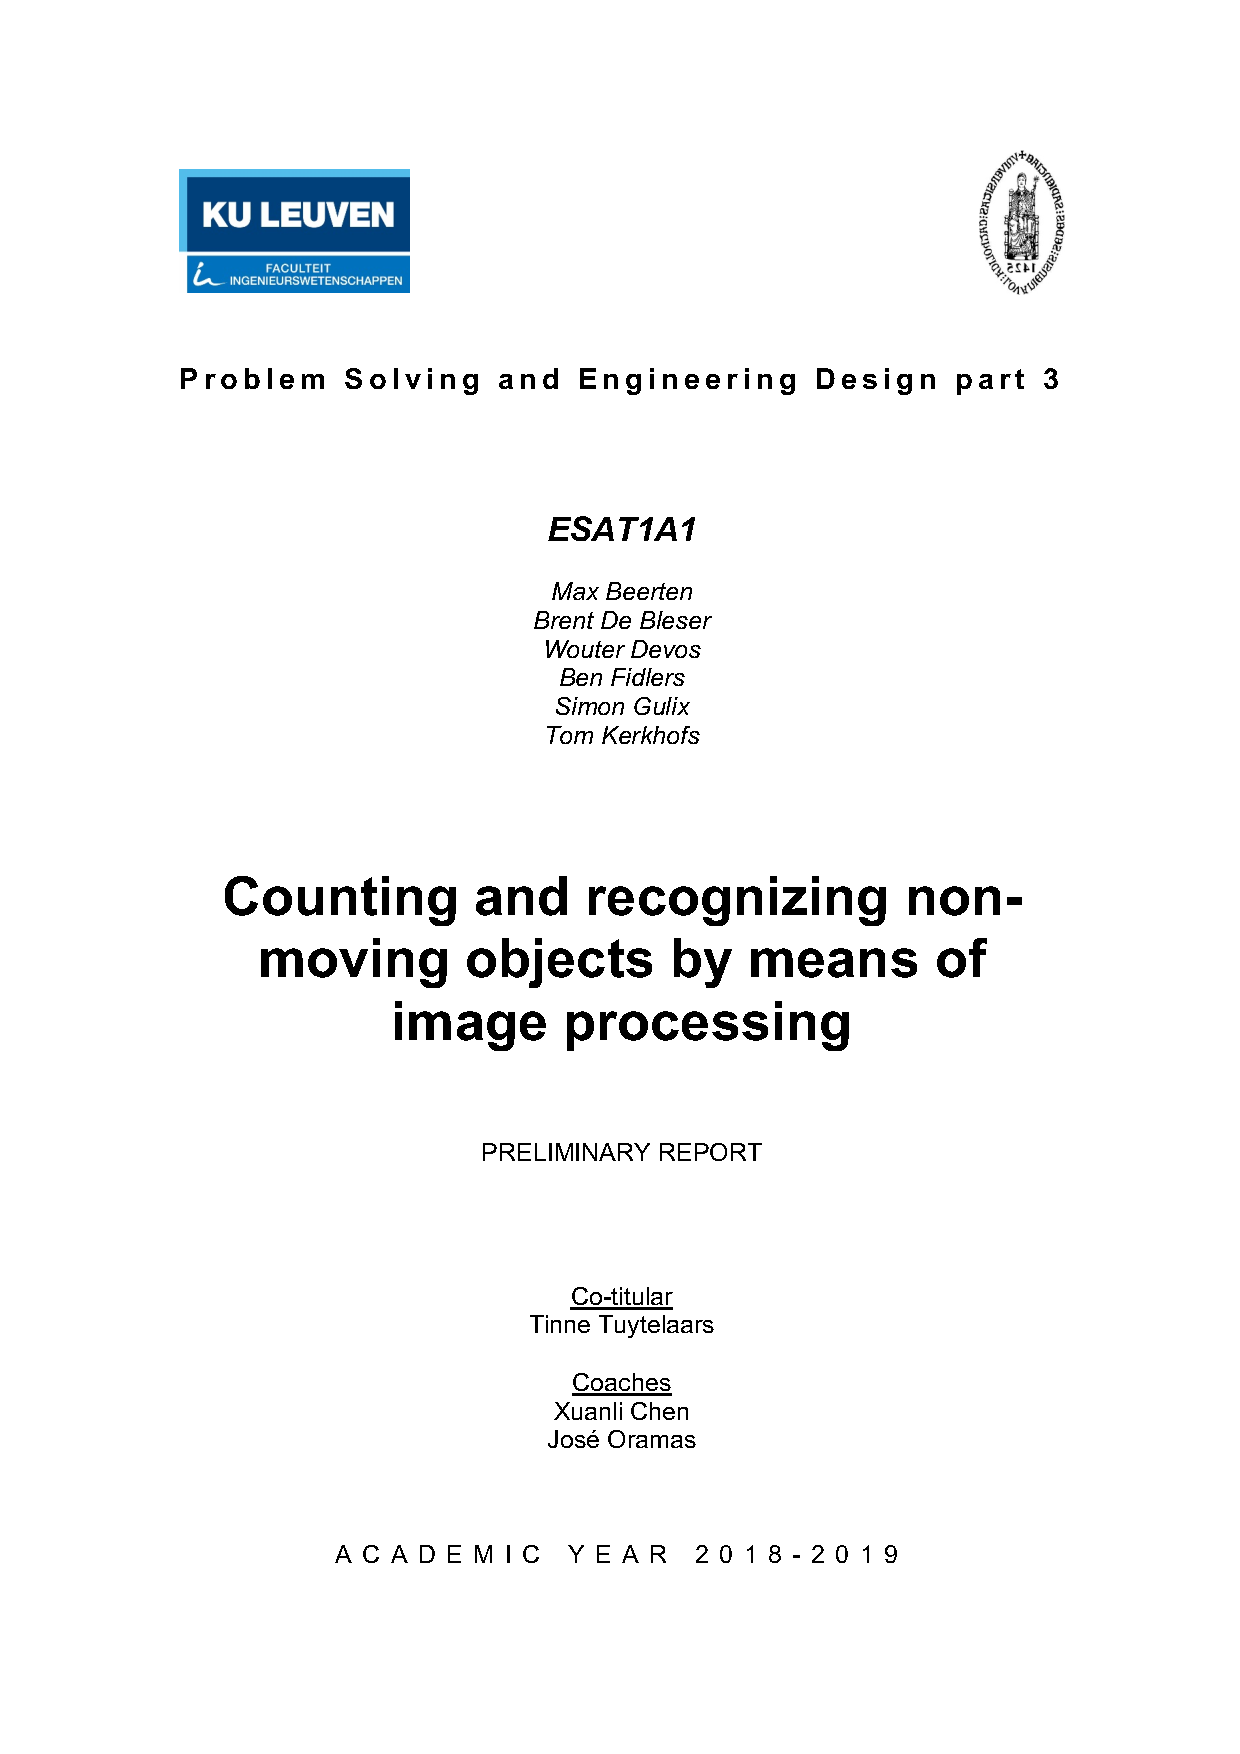
\includepdf[pages=-]{frontpage.pdf}

\section*{Abstract}
\thispagestyle{empty}

\newpage
\tableofcontents
\thispagestyle{empty}

\newpage
\listoftables
\thispagestyle{empty}

<<<<<<< HEAD
\tableofcontents

\section{List of tables and figures}
hier komt een lijst van tabellen, figuren en afkortingen
=======
\newpage
\listoffigures
\thispagestyle{empty}
>>>>>>> 8145d2b07a6d6c4afd0f49acb564e72f68fa6068

\newpage
\section{Introduction}
\pagenumbering{arabic}

\section{Description of the problem}

\noindent Given is a basket with a standard rectangular shape with fixed dimensions. The objective is to count every object in this basket. If possible, the objects can be outlined by the system. An optional objective was to be able to measure the objects in the basket.\\

\noindent The system used should be based on colour and depth images. The objects won't have the same colour as the basket and/or have a noticeable depth. Otherwise the camera can't notice the objects. the project had to be made with a budget of \euro 250.


\section{Design and implementation}
\subsection{Hardware}
\subsection{Software}
\subsubsection{RGB sensor}

There are a lot of options when it comes to software and there exist many different algorithms for image processing. The diagram on FIG…XX… shows a couple of different methods. There is no ‘right-way’ to count objects in an image. Different methods have different advantages and disadvantages. The only things that appears in almost all algorithms are:
-	Converting the RGB image to grayscale
-	Run filters over the image to remove noise
These things are also visible in the diagram.
Method 1
This method is the most simple and easy to write. It starts with the grayscale image which has been filtered. Then it runs an thresholding-algorithm with a pre-defined threshold value over the image and the output is a binary image. That’s an image that only has 0’s and 1’s in his matrix.  It’s also possible to use an algorithm to search for the best threshold value.  After that there is a simple edge detection algorithm which makes the edges visible. 
Advantages: it’s an easy and fast algorithm.
Disadvantages: with a pre-defined threshold value it just classifies pixels based on colour. 
Method 2
Method 2 is the reverse of method 1: it starts with an edge detection algorithm. But a different one than in method 1 and a bit more complicated. This algorithm gives back an greyscale image, not a binary image. After that is a threshold algorithm with a pre-defined threshold value and the edges are converted to a binary image. Because there is a lot of noise with this method, it's recommended to use a noise reduction algorithm. 
Advantages: it detects all kind of objects, not based on colour or shape.
Disadvantages: the boundary between different objects needs to be clear.
Method 3
This method is different. It makes a compromise in functionality: it needs a picture of the background alone before it can detect objects. First it loads an background image, converts it to grayscale and runs some filters over the image. After that, the algorithm loops through the image pixel by pixel, checks if the pixel on the image is within a certain range of the same pixel on the background image. If the pixel is within that range, that pixel gets classified as background. The output is a binary image with only the objects.  
Advantages: it is better in detecting objects, not based on colour or shape.
Disadvantages: There needs to be an image of the empty background, and lightning conditions etc. can’t change.


\subsubsection{Depth sensor}

\section{Budget management}

\section{course integration}

\section{Conclusion}

\section{List of references}

\section{Appendix}

\end{document}
